
%\documentclass{vgtc}
\documentclass[journal]{vgtc}                % final (journal style)
%\documentclass[review]{vgtc}                 % review
%\documentclass[review,journal]{vgtc}         % review (journal style)
%\documentclass[widereview]{vgtc}             % wide-spaced review
%\documentclass[preprint]{vgtc}               % preprint
%\documentclass[preprint,journal]{vgtc}       % preprint (journal style)
%\documentclass[electronic]{vgtc}             % electronic version
%\documentclass[electronic,journal]{vgtc}     % electronic version, journal

%% Uncomment one of the lines above depending on where your paper is
%% in the conference process. ``review'' and ``widereview'' are for review
%% submission, ``preprint'' is for pre-publication, and the final version
%% doesn't use a specific qualifier. Further, ``electronic'' includes
%% hyperreferences for more convenient online viewing.

%% Please use one of the ``review'' options in combination with the
%% assigned online id (see below) ONLY if your paper uses a double blind
%% review process. Some conferences, like IEEE Vis and InfoVis, have NOT
%% in the past.

%% These three lines bring in essential packages: ``mathptmx'' for Type 1
%% typefaces, ``graphicx'' for inclusion of EPS figures. and ``times''
%% for proper handling of the times font family.
%% We encourage the use of mathptmx for consistent usage of times font
%% throughout the proceedings. However, if you encounter conflicts
%% with other math-related packages, you may want to disable it.

\usepackage{mathptmx}
\usepackage{graphicx}
\usepackage{times}
%\usepackage{tabularx}
\usepackage{amsmath}
%\usepackage{url}
\usepackage{subfigure}
\usepackage{multirow}

%% If you are submitting a paper to a conference for review with a double
%% blind reviewing process, please replace the value ``0'' below with your
%% OnlineID. Otherwise, you may safely leave it at ``0''.
\onlineid{0}

%% declare the category of your paper, only shown in review mode
\vgtccategory{Research}

%% allow for this line if you want the electronic option to work properly
\vgtcinsertpkg

%% In preprint mode you may define your own headline.
%\preprinttext{To appear in an IEEE VGTC sponsored conference.}

\usepackage{color}
\definecolor{RED}{rgb}{1,0,0}
\definecolor{BLUE}{rgb}{0,0,1}
\newcommand{\FIXME}[1]{\textbf{\color{BLUE}{FIXME: #1}}}
\newcommand{\sref}[1]{Section~\ref{#1}}
%\newcommand{\FIXME}[1]{}

% suppress  single floating lines on top (widow) and bottom (club)
%  10000 is infinity
%  tradeoff: possible underful vboxes
\clubpenalty=10000
\widowpenalty=10000

%% Paper title.
%----------------------------------------------------------------------
\title{Equalizer: A Mature Parallel Rendering Framework}
%----------------------------------------------------------------------

%% Author and Affiliation (multiple authors with multiple affiliations)
\author{Stefan Eilemann\thanks{email: eilemann@gmail.com} \\ %
\and Renato Pajarola\thanks{email: pajarola@acm.org}}

\affiliation{\scriptsize Visualization and MultiMedia Lab \\ Department of Informatics \\ University of Z\"urich}

%% Keywords that describe your work. Will show as 'Index Terms' in journal
%% please capitalize first letter and insert punctuation after last keyword
\keywords{Parallel Rendering, Scalable Visualization, Cluster Graphics, Immersive Environments, Display Walls}

%% ACM Computing Review (CR) categories.
%% See <http://www.acm.org/class/1998/> for details.
%% The ``\CRcat'' command takes four arguments.

\CRcatlist{ % not used in journal version
  \CRcat{I.3.2}{Graphics Systems}{Distributed Graphics}{Parallel Rendering};
  \CRcat{I.3.m}{Miscellaneous}{Rendering Clusters}{Scalable Rendering};
  \CRcat{I.3.7}{Three-Dimensional Graphics and Realism}{Virtual Reality}{Immersive Environments}
}

\vgtccategory{Research}

%% Copyright space is enabled by default as required by guidelines.
%% It is disabled by the 'review' option or via the following command:
% \nocopyrightspace

%%%%%% START OF THE PAPER %%%%%%
\begin{document}

%----------------------------------------------------------------------
%% Abstract section.
\abstract{ We present the features, algorithms and system integration necessary
  to implement a parallel rendering framework usable in a wide range of
  real-world research and industry applications, based on the basic architecture
  and implementation of the Equalizer parallel rendering framework presented in
  \cite{EMP:09}.  } % end of abstract

\maketitle

\begin{figure*}[ht]\center
  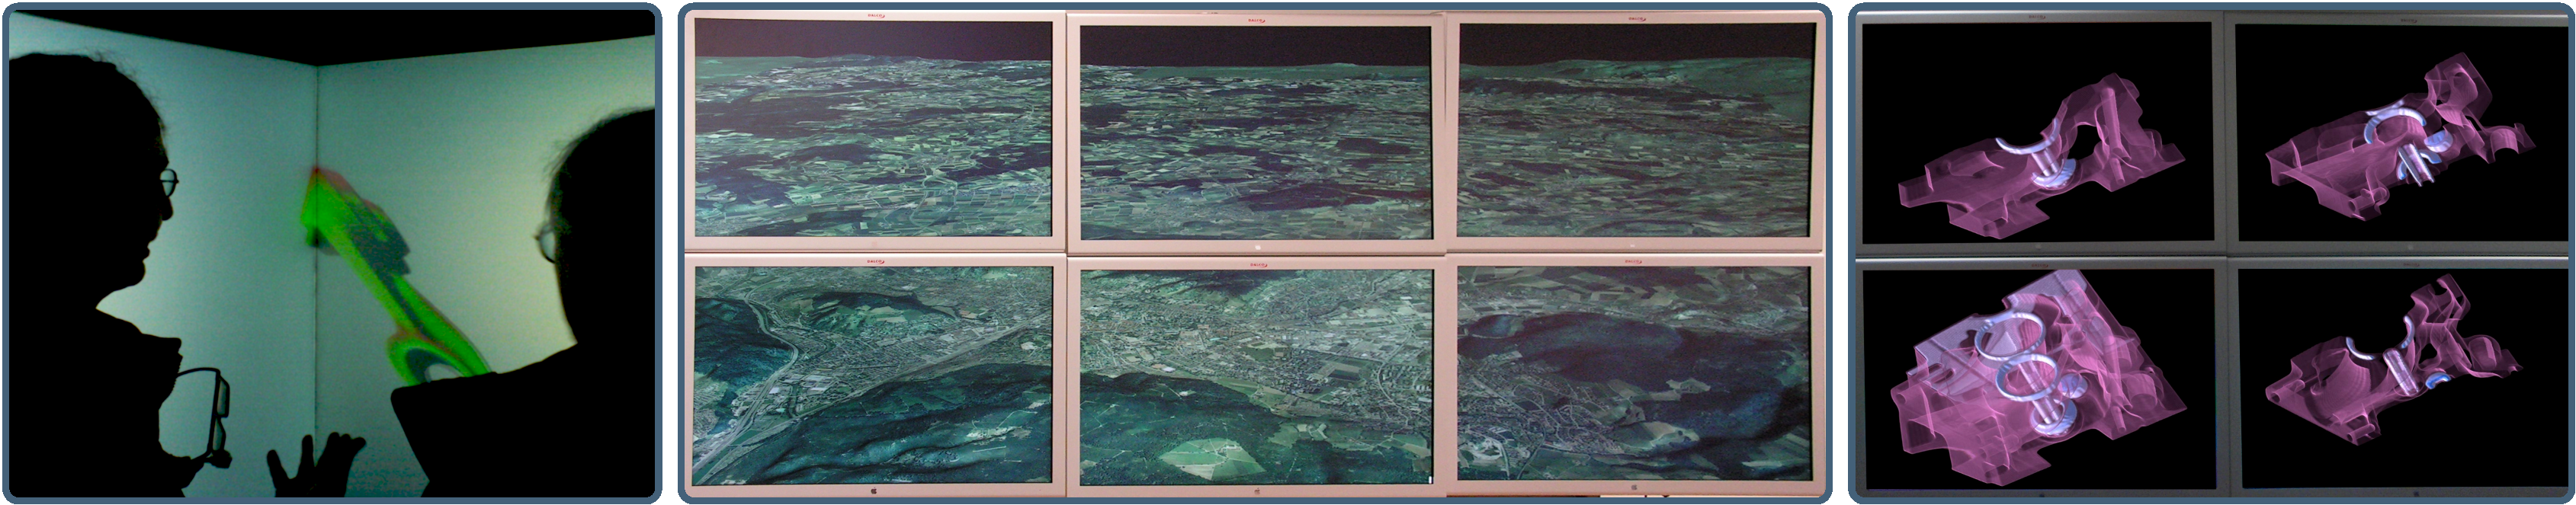
\includegraphics[width=2\columnwidth]{images/teaser} \\
  (a) \hfil \hfil (b) \hfil \hfil (c)
  \vspace{-2mm}
  \caption{Example Equalizer application use cases: (a) 192 Megapixel CAVE at
    KAUST running RTNeuron, (b) Immersive HMD with external tracked and
    untracked views running RTT DeltaGen for virtual car usability studies (c)
    Cave2 running a molecular visualization build using Omegalib.}
  \label{FIG_teaser}
\end{figure*}

%----------------------------------------------------------------------
\section{Introduction}
%----------------------------------------------------------------------

The continuing improvements in hardware integration lead to ever faster CPUs and GPUs, as well as higher resolution sensor and display devices. Moreover, increased hardware parallelism is applied in form of multi-core CPU workstations, massive parallel super computers, or cluster systems. Hand in hand goes the rapid growth in complexity of data sets from numerical simulations, high-resolution 3D scanning systems or bio-medical imaging, which causes interactive exploration and visualization of such large data sets to become a serious challenge. It is thus crucial for a visualization solution to take advantage of hardware accelerated scalable parallel rendering. In this systems paper we describe a new scalable parallel rendering framework called {\em Equalizer} that is aimed primarily at cluster-parallel rendering, but works as well in a shared-memory system. Cluster systems are the main focus  because workstation graphics hardware is developing faster than high-end graphics (super-) computers can absorb new developments, and also because clusters offer a better cost-performance balance.

Previous parallel rendering approaches typically failed in one of the following system requirements:
%
\begin{enumerate}\renewcommand{\labelenumi}{\alph{enumi})}
\addtolength{\itemsep}{-0.5\baselineskip}
\item generic application support, instead of special domain solution
\item scalable abstraction of the graphics layer
\item exploit existing code infrastructure, such as proprietary scene graphs, molecular data structures, level-of-detail and geometry databases
\end{enumerate}

To date, generic and scalable parallel rendering frameworks  that can be adopted to a wide range of scientific visualization domains are not yet readily available. Furthermore, flexible
configurability to arbitrary cluster and display-wall configurations has also not been addressed in the past, but is of immense practical importance to scientists depending high-performance interactive visualization as a scientific tool. In this paper we present Equalizer, which is a novel flexible framework for parallel rendering that supports scalable performance, configuration flexibility, is {\em minimally invasive} with respect to adapting existing visualization applications, and is applicable to virtually any scientific visualization application domain.

The main contributions that Equalizer introduces in a single parallel rendering system, and which are presented in this paper are:
%
\begin{enumerate}\renewcommand{\labelenumi}{\roman{enumi})}
\addtolength{\itemsep}{-0.5\baselineskip}
\item novel concept of compound trees for flexible configuration of graphics system resources,
\item easy specification of parallel task decomposition and image compositing choice through compound tree layouts,
\item automatic decomposition and distributed execution of rendering tasks according to compound tree,
\item support for parallel surface as well as transparent (volume) rendering through $z$-visibility as well as $\alpha$-blending compositing,
\item fully decentralized architecture providing network swap barrier (synchronization) and distributed objects functionality,
\item support for low-latency distributed frame synchronization and image compositing,
\item minimally invasive programming model.
\end{enumerate}

Equalizer is open source, available under the LGPL license from http://www.equalizergraphcis.com/, which allows it to be used both for open source and commercial applications. It is source-code portable, and has been tested on Linux, Microsoft Windows, and Mac OS X in 32 and 64 bit mode using both little endian and big endian processors.


%----------------------------------------------------------------------
\section{Related Work}
%----------------------------------------------------------------------
\label{SEC_related}

\cite{EMP:09} summarized the work in parallel rendering at the time of
publication. In the following we will present the related work published since
this publication.

\cite{EEP:11} cross-segment load balancing

\cite{DK:11}: Framework to develop apps for multitile, thus targeted
specifically for tiled-wall visualization systems: grid configuration,
scalability (?), multiple work sessions, multiuser events. Master-slave approach
like Eq. with grid nodes running instances of the application. Is maybe more
like a GLUT and window replacement, or enhancement to deal with the OpenGL
contexts and events

\cite{CKP:12} tiled display wall virtual environment

\cite{TBD} DisplayCluster

\cite{NHM:11} ClusterGL?

Omegalib

%------------------------------------------------------------------------------
\section{Usability}
%------------------------------------------------------------------------------

In this section we present features motivated by real-world application use
cases, i.e., new functionalities rather then performance improvements. We
motivate the use case, explain the architecture and integration into our
parallel rendering framework, and, where applicable, show the steps needed to
use this functionality in applications.

\subsection{Physical and Logical Visualization Setup}

Real-world visualization setups are often complex, and having an abstract
representation of the display system can simplify the configuration
process. Real-world applications often have the need to be aware of spatial
relationship of the display setup, for example to render 2D overlays or to
configure multiple views on a tiled display wall.

We addressed this need through a new configuration section interspersed between
the node/pipe/window/channel hardware resources and the compound trees
configurating the resource usage for parallel rendering.

A typical installation consists of one projection canvas, which is one
aggregated projection surface, e.g., a tiled display wall or a CAVE. Desktop
windows are considered a canvas. Each canvas is made of one or more segments,
which are the individual outputs connected to a display or projector. Segments
can be planar or non-planar to each other, and can overlap or have gaps between
each other. A segment is referencing a channel, which defines the output area of
this segment, e.g., on a DVI connector connected to a projector.

A canvas can define a frustum, which will create default, planar sub-frusta for
all of its segments. A segment can also define a frustum, which overrides the
canvas frustum, e.g., for non-planar setups such as CAVEs or curved
screens. These frusta describe a physically-correct display setup for a Virtual
Reality installation. A canvas may have a software or hardware swap barrier,
which will synchronize the rendering of all contributing GPUs.

On each canvas, the application can display one or more views. A view is a view
on a model, in the sense used by the MVC pattern. The view class is used by
Equalizer applications to define view-specific data for rendering, e.g., a
scene, viewing mode or camera. The application process manages this data, and
the render clients receive it for rendering.

A layout groups one or more views which logically belong together. A layout is
applied to a canvas. The layout assignment can be changed at run-time by the
application. The intersection between views and segments defines which output
channels are available, and which frustum they should use for rendering. These
output channels are then used as destination channels in a compound. They are
automatically created during configuration.

A view may have a frustum description. The view's frustum overrides frusta
specified at the canvas or segment level. This is used for non-physically
correct rendering, e.g., to compare two models side-by-side on a tiled display
wall. If the view does not specify a frustum, the corresponding destination
channels will use the physically correct sub-frustum resulting from the
view/segment intersection.

An observer looks at one or more views. It is described by the observer position
in the world and its eye separation. Each observer will have its own stereo
mode, focus distance and frame loop (framerate). This allows to have untracked
views and multiple tracked views, e.g., two HMDs, in the same application.

\subsection{Automatic Configuration}

Automatic configuration implements the discovery of local and remote resources
as well as the creation of typical configurations using the discovered resources
at application launch time.

The discovery is implemented in a separate library, hwsd (HardWare Service
Discovery), which uses a plugin-based approach to discover GPUs for GLX, AGL or
WGL windowing systems, as well as network interfaces on Linux, Mac OS X and
Windows. Furthermore, it detects the presence of VirtualGL to allow optimal
configuration of remote visualization clusters. The resources can be discovered
on the local workstation, and through the help of a simple daemon using the
zeroconf protocol, on a set of remote nodes within a visualization cluster. A
session identifier may be used to support multiple users on a single cluster.

The Equalizer server uses the hwsd library to discover local and remote
resources when an hwsd session name instead of a \textsf{.eqc} configuration
file is provided. A set of standard decomposition modes is configured, which can
be selected through activating the corresponding layout.

This versatile mechanism allows non-experts to configure asnd profit from
multi-GPU workstations and visualization clusters, as well as to provide system
administrators with the tools to implement easy to use integration with cluster
schedulers. This feature is transparent to Equalizer application developers.

\subsection{Qt Windowing}

Challenges in threading model, architecture

\subsection{Tide Integration}

Tiled interactive display environment, parallel pixel streaming, events

\subsection{Sequel}

application, renderer, view data

%------------------------------------------------------------------------------
\section{The Collage Network Library}
%------------------------------------------------------------------------------

\subsection{Distributed, Versioned Objects}

types (instance, delta, static), versioning, multicast, compression,
serializable with dirty bits, mapping, blocking commits

\subsection{Reliable Stream Protocol}

UDP-based reliability protocol

\subsection{Infiniband RDMA}

reverse-engr impl

%------------------------------------------------------------------------------
\section{Virtual Reality}
%------------------------------------------------------------------------------

\subsection{Dynamic Focus Distance}

Focus what user is looking at

\subsection{Asymmetric Eye Position}

Better HMD by measuring user geometry

\subsection{Application-specific Scaling}

Gullivers world

\subsection{Runtime Stereo Switch}

\subsection{Swap Synchronization and GPU affinity}

%------------------------------------------------------------------------------
\section{Performance}
%------------------------------------------------------------------------------

\subsection{New Decomposition Modes}

The initial version of Equalizer implemented sort-first (2D), sort-last (DB) and
stereo (EYE) decomposition. In the following we present new decomposition modes
and motivate their use case.

\subsubsection{Time-Multiplex}

Time-multiplexing, or DPlex, was already implemented in \cite{BRE:05}. While it
increases the framerate linearly, it does not decrease the latency between user
input and the corresponding output. Consequently, this decomposition mode is
mostly useful for non-interactive movie generation. It is transparent to
Equalizer applications, but does require the configuration latency to be equal
or greater than the number of source channels. Furthermore, to work in a
multi-threaded, multi-GPU configuration, the application needs to support
running the rendering threads asynchronously, as outlined in
\sref{SEC_threading}.

\subsubsection{Tiles and Chunks}

Tile and chunk decompositions are a variant of sort-first and sort-last
rendering, respectively. They decompose the scene into a predefined set of
fixed-size image tiles or database ranges. These tasks are queued and processed
by all source channels by polling a server-central queue. Prefetching ensures
that the task communication overlaps with rendering. As shown in \cite{SPEP:16},
these modes provide better performance due to being inherently load-balanced, as
long as there is an insignificant overhead for the render task setup. This mode
is transparent to Equalizer applications.

\subsubsection{Pixel}

Pixel compounds decompose the destination channel by interleaving rows or
columns in image space. They are a variant of sort-first decomposition which
works well for fill-limited applications which are not geometry bound. Source
channels cannot reduce geometry load through view frustum culling, since each
source channel has almost the same frustum (only shifted by some pixels),
but applied to a reduced 2D viewport. However, the fragment load on all source
channels is very similar due to the interleaved distribution of pixels. This
functionality is transparent to Equalizer applications, and the default
compositing implementation uses the OpenGL stencil buffer to blit pixels onto
the destination channel.

\subsubsection{Subpixel}

Subpixel compounds are similar to pixel compounds, but they decompose the work
for a single pixel, for example when using multisampling or depth of
field. Composition typically uses accumulation and averaging of all computed
fragments for a pixel. This feature is not fully transparent to the application,
since it needs to adapt (jitter or tilt) the frustum based on the iteration
executed. Furthermore, subpixel compounds interact with idle image refinements,
e.g., they can accelerate idle anti-aliasing of a scene when the camera and
scene are not changed.

\subsection{Equalizers}

Equalizer are an addition to compound trees. They modify parameters of their
respective subtree at runtime to optimize one aspect of the decomposition.

\subsubsection{Sort-First and Sort-Last Load Equalizer}

reactive load equalization, describe tunables (damping, resistance, delta,
granularity), sort-first respects input channel size

\subsubsection{Cross-Segment Load Equalizer}

summarize \cite{EEP:11}

\subsubsection{Dynamic Frame Resolution}

Constant frame rate for fill-limited applications

\subsubsection{Frame Rate Equalizer}

Predominantly used by DPlex to smooth output framerate

\subsubsection{Monitoring}

Control workstation in VR setups

\subsection{Optimizations}

\subsubsection{Region of Interest}

The region of interest is the screen-space 2D bounding box enclosing the
geometry rendered by a single resource. We have extended the core parallel
rendering framework to use an application-provided ROI to optimize the load
equalizer as well as image compositing performance. The load equalizer uses the
ROI to refine its load grid to the regions containing data. The compositing code
uses the ROI to minimize image readback and network transmission. In
\cite{EBAHMP:12}, we provide the details of the algorithm, and show that this
improves rendering performance of up to 25\%.

\subsubsection{Asynchronous Compositing}

Asynchronous compositing pipelines rendering with compositing operations, by
executing the image readback, network transfer and image assembly from threads
running in parallel to the rendering threads. In \cite{EBAHMP:12}, we provide
the details of the implementation and experimental data showing an improvement
of the rendering performance of over 25\% for large node counts.

\subsubsection{Download and Compression Plugins}

GPU-CPU transfer plugins with optional compression (eg YUV) linked to CPU
compression for network transfer

\subsubsection{Thread Synchronization Modes}\label{SEC_threading}

Per-node sync, draw sync, async

%----------------------------------------------------------------------
\section{Applications}
%----------------------------------------------------------------------

\subsection{Livre}
\subsection{RTT Deltagen}

\subsection{RTNeuron}
\cite{HBBES:13}

\subsection{Raster}
\subsection{Omegalib}

%----------------------------------------------------------------------
\section{Experimental Results}
%----------------------------------------------------------------------
\label{SEC_results}

\subsection{Object Distribution}

Distribute large ply model to 1..16 nodes using TCP, IB and RSP

\subsection{Decomposition Modes}

Two graphs: Time to render a 4k, 256-step MSAA image of largest ply model and
Livre using 1..16 nodes with all modes (2D, 2D LB, DB, DPlex (over AA steps),
tiles, chunks, pixel, subpixel)

%----------------------------------------------------------------------
\section{Discussion and Conclusion}
%----------------------------------------------------------------------
\label{SEC_conclusions}


%----------------------------------------------------------------------
%\section*{Acknowledgements}
%----------------------------------------------------------------------
%% if specified like this the section will be ommitted in review mode
\acknowledgements{
We would like to thank and acknowledge the following institutions and projects for providing the 3D geometry and volume test data sets:
the Digital Michelangelo Project, Stanford 3D Scanning Repository, Cyberware Inc., volvis.org and the Visual Human Project.
This work was partially supported by the Swiss National Science Foundation Grant 200021-116329/1.
}

\vspace{-2mm}
\footnotesize
\bibliographystyle{abbrv}
\bibliography{references}

\end{document}
